
\subsubsection{Cadre Général}

Le module d'introspection a pour objectif d'extraire, à partir des expériences passées de l'IA, de nouvelles formes remarquables potentiellement discriminante pour les choix futurs. Pour ce faire, il choisi aléatoirement, en mémoire, au moins deux environnements ayant reçu la même annotations et tente d'étendre les formes déjà connues.

\begin{figure}[H] 
\begin{center}
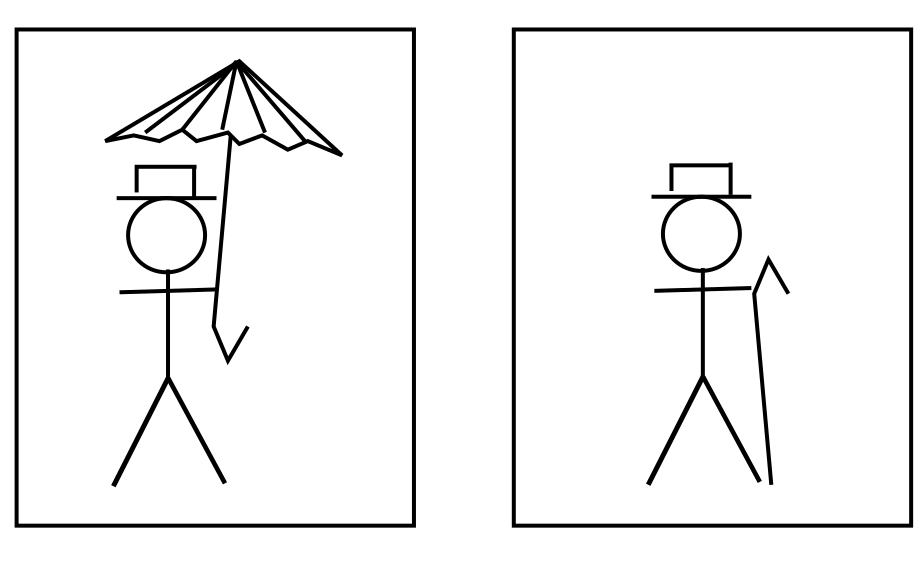
\includegraphics[width=0.8\textwidth]{files/raisonneur/reconnaissance_de_formes_0} 
\end{center}
\caption{Illustration de la reconnaissance de forme} 
\label{img_reco_forme_0}
\end{figure}

Par exemple, sur la figure \ref{img_reco_forme_0}, nous considérons deux environnements présents en mémoire. Le premier représentant un homme avec un chapeau et un parapluie, le second un homme avec un chapeau et une canne. Nous souhaitons extraire de ces deux environnements la forme \og homme avec un chapeau \fg{}. Pour ce faire, ce module se base, sur les connaissances, présentent en mémoire relatives à ces environnements. En l'occurrence, nous considérerons que notre IA sait déjà reconnaître un homme et les a reconnu sur ces environnements. Notre module cherche alors à étendre, le plus possible, la forme \og homme \fg dans un des deux environnements tout en vérifiant que cette forme étendu peux toujours être injectée dans l'autre environnement, comme illustré dans la figure \ref{img_reco_forme_injection}.

\begin{figure}[H] 
\begin{center}
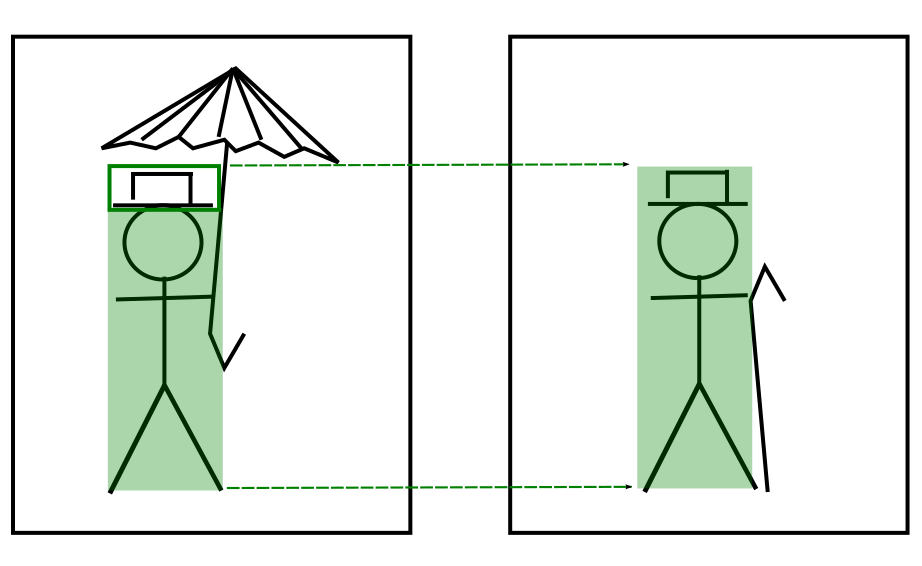
\includegraphics[width=0.8\textwidth]{files/raisonneur/reconnaissance_de_formes_injection} 
\end{center}
\caption{Illustration de l'injection} 
\label{img_reco_forme_injection}
\end{figure}

\subsubsection{Application aux jeux de plateau}

\begin{figure}[H] 
\begin{center}
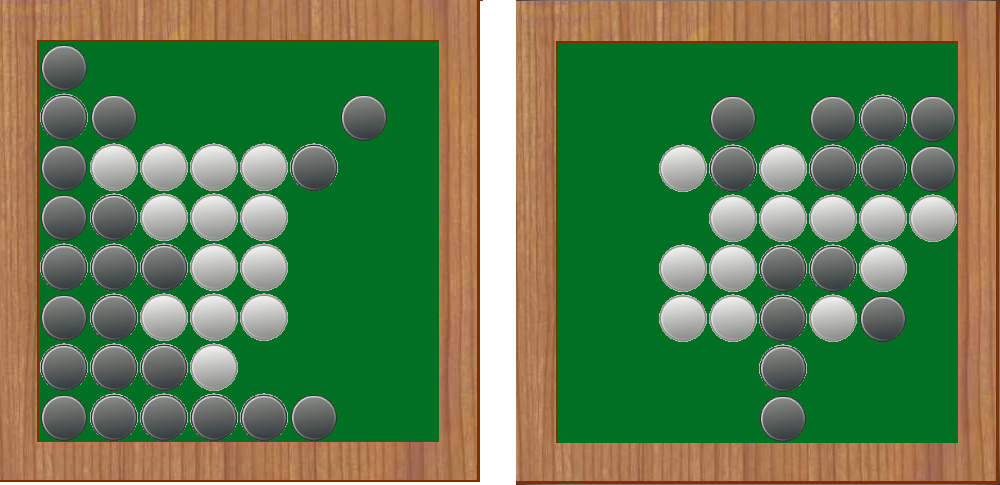
\includegraphics[width=0.7\textwidth]{files/raisonneur/cbs_reco0} 
\end{center}
\caption{Illustration de l'injection} 
\label{img_cbs_reco0}
\end{figure}

\begin{figure}[H] 
\begin{center}
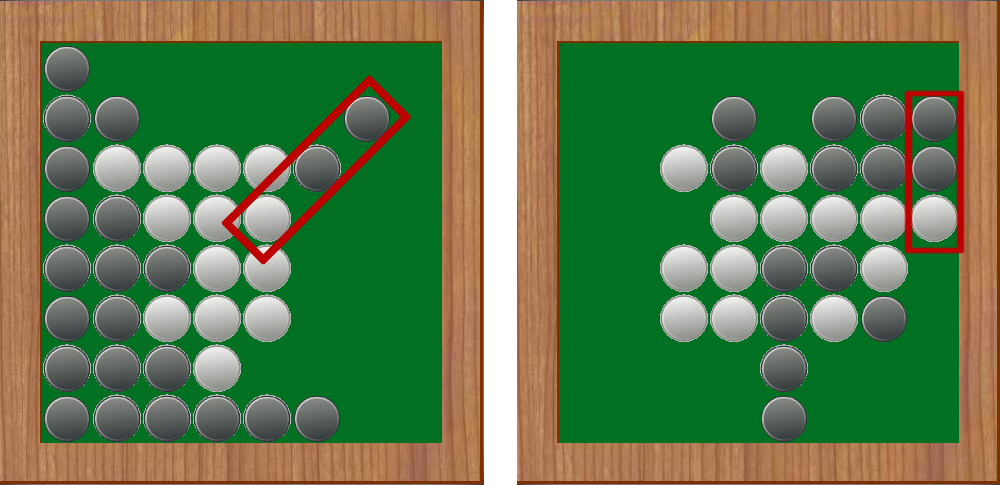
\includegraphics[width=0.7\textwidth]{files/raisonneur/cbs_reco1} 
\end{center}
\caption{Illustration de l'injection} 
\label{img_cbs_reco1}
\end{figure}

\begin{figure}[H] 
\begin{center}
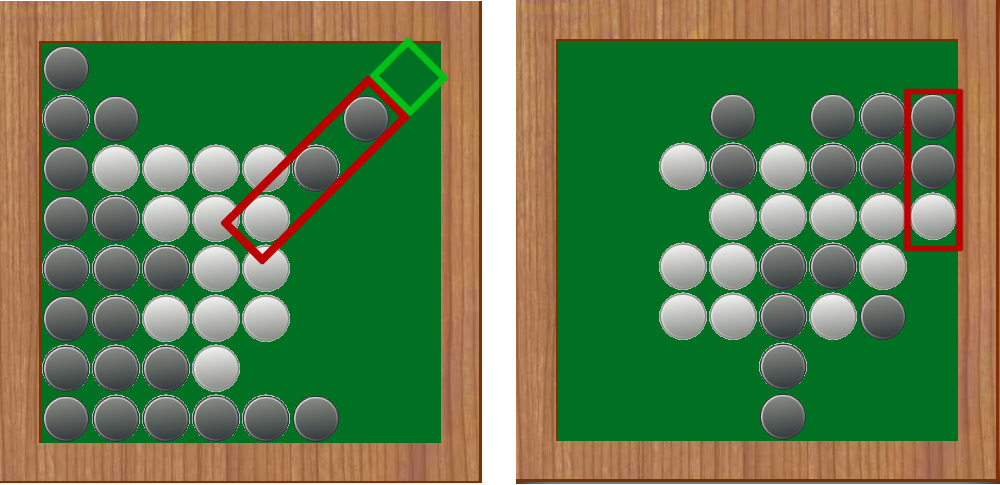
\includegraphics[width=0.7\textwidth]{files/raisonneur/cbs_reco2} 
\end{center}
\caption{Illustration de l'injection} 
\label{img_cbs_reco2}
\end{figure}

\begin{figure}[H] 
\begin{center}
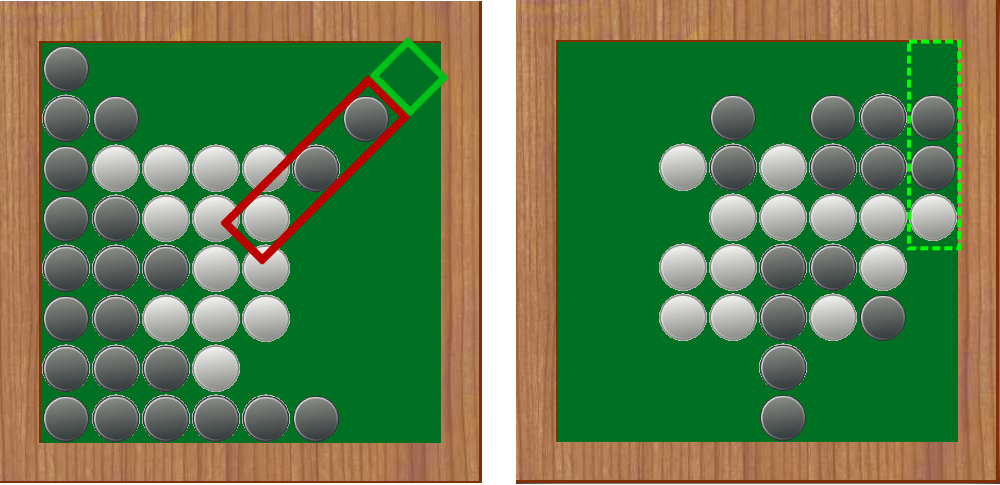
\includegraphics[width=0.7\textwidth]{files/raisonneur/cbs_reco3} 
\end{center}
\caption{Illustration de l'injection} 
\label{img_cbs_reco3}
\end{figure}